		\subsection{ระยะทาง การกระจัด อัตราเร็ว และความเร็ว}
		\begin{minipage}{\textwidth}
			\begin{tabbing}
				\textbf{ระยะทาง} \quad \=\textbf{คือ} ความยาวตามแนวที่เคลื่อนที่ได้จริง มีหน่วยเป็นเมตร (m) \\
				\textbf{การกระจัด} 		\>\textbf{คือ} \=ความยาวที่วัดเป็นเส้นตรงจากจุดเริ่มต้นถึงจุดสุดท้ายของ\\
														\>\>การเคลื่อนที่มีหน่วยเป็นเมตร (m)
			\end{tabbing}
			\adjustbox{valign=t}{
				\begin{minipage}[t]{0.6\linewidth}
					\textbf{ตัวอย่างเช่น} หากวัตถุก้อนหนึ่งเคลื่อนที่จากจุด A  ไปจุด B  แล้วเคลื่อนต่อไปจุด C  ในทิศที่ตั้งฉากกันดังรูป   จะได้ว่า	
					\begin{align*}
						\text{ระยะทาง} &= \text{ตามแนวที่เคลื่อนที่ได้จริง} \\
						\text{ระยะทาง} &= 4 + 3 \text{เมตร} \\
						\text{ระยะทาง} &= 7 \text{เมตร}	\quad \text{\textbf{*** ไม่ต้องสนใจทิศทาง}}
					\end{align*}
				\end{minipage}
			}%
			\hfill
			\adjustbox{valign=t}{
				\begin{minipage}[t]{0.3\linewidth}
	    			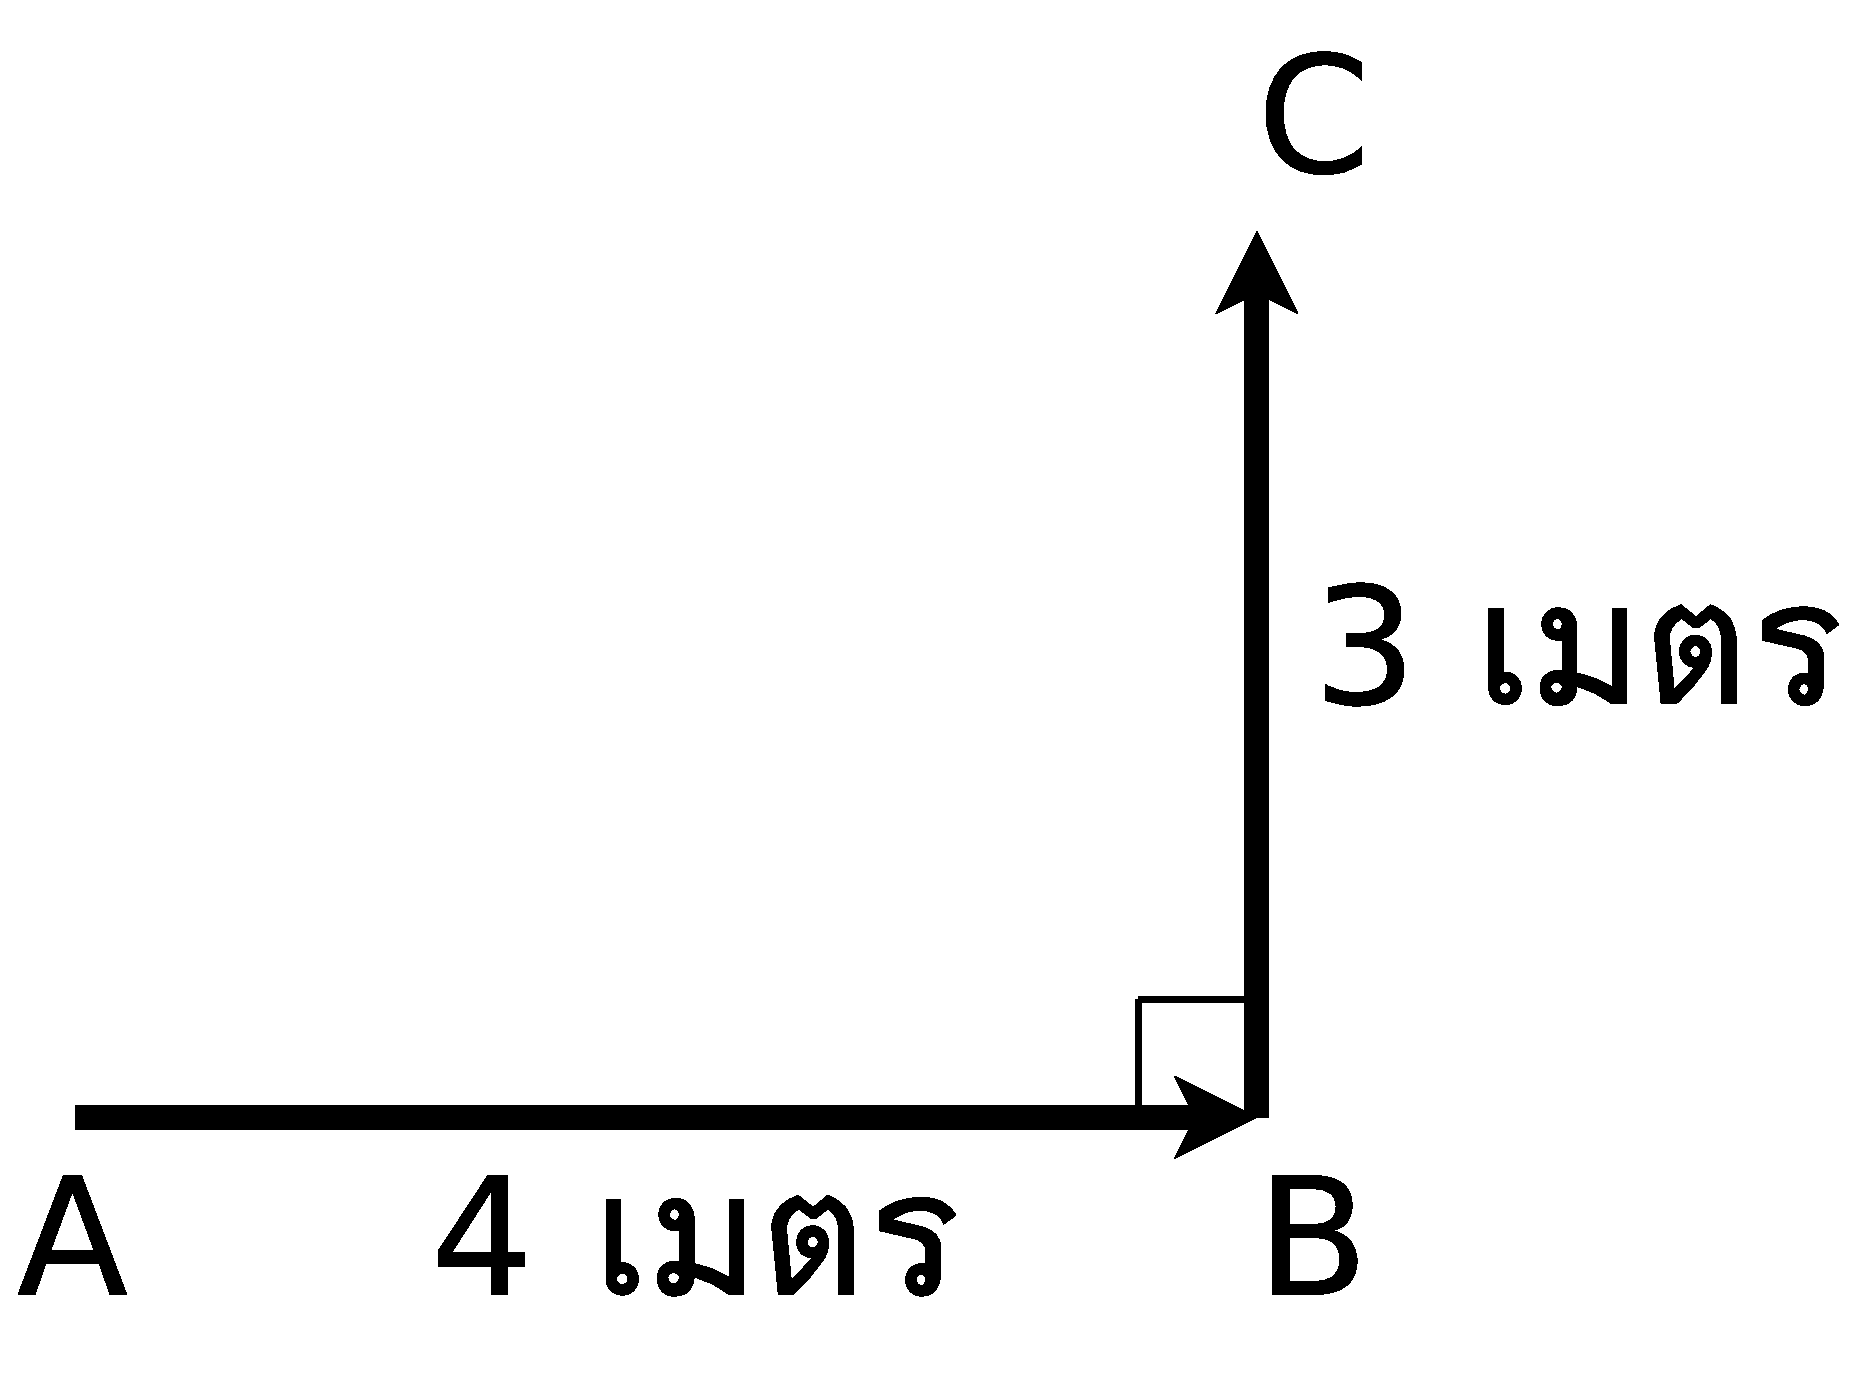
\includegraphics[width=\linewidth]{pic1.eps}
				\end{minipage}
			}
		\end{minipage}
		\begin{minipage}{\textwidth}
					\textbf{และจะได้อีกว่า}\\
			\adjustbox{valign=t}{
				\begin{minipage}[t]{0.6\linewidth}
					\begin{tabbing}
						การกระจัด \= $=$ \=ความยาวที่วัดเป็น\underline{เส้นตรง}จาก \\
									\>\>จุดเริ่มต้นถึงจุดสุดท้าย \\
						การกระจัด \> $=$ 5  \text{เมตร} 
					\end{tabbing}
				\end{minipage}
			}%
			\hfill
			\adjustbox{valign=t}{
				\begin{minipage}[t]{0.3\linewidth}
	    			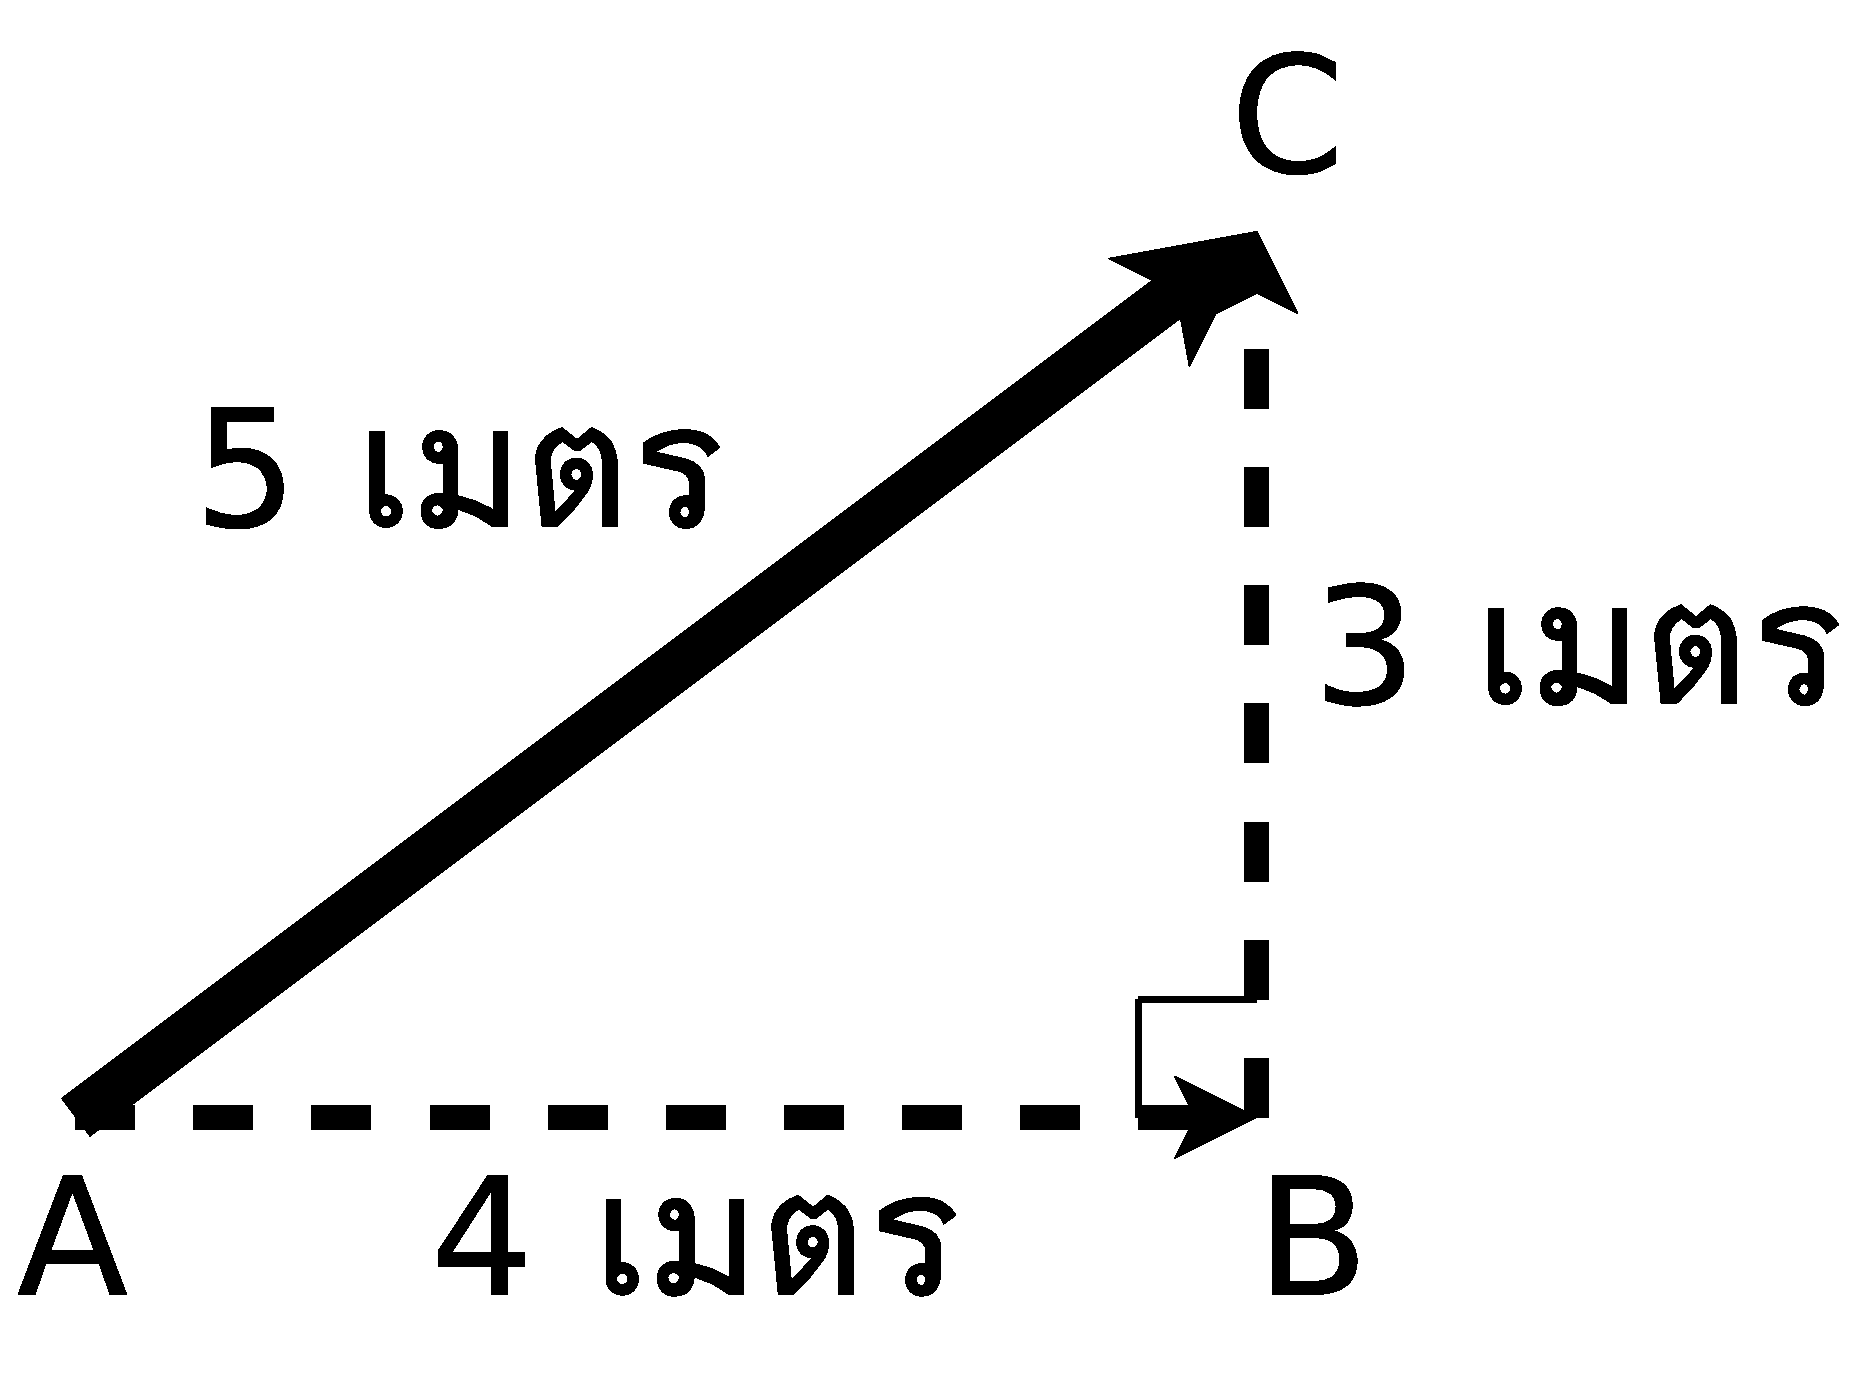
\includegraphics[width=\linewidth]{pic2.eps}
				\end{minipage}
			}	
			\begin{center}
				\textbf{*** การกระจัดนี้มีทิศจากจุดเริ่มต้น (A) ไปถึงจุดสุดท้าย (C)}
			\end{center}
		\end{minipage}
